\documentclass{article}
\usepackage{graphicx}
\usepackage{amsmath}
\usepackage{cite}
\usepackage{color}
\usepackage{enumitem}
\usepackage{natbib}
\usepackage{tabularx}
\usepackage{natbib}
\usepackage{ragged2e}
\usepackage{geometry}
\geometry{a4paper, left=3.5 cm, right=3.5 cm, top=3 cm, bottom=3 cm}

\title{\huge\textbf{La digitalizzazione nelle PA}}
\author{\texttt{Alessandro Meloni 0001118676 GEPID}}
\date{Anno accademico 2023/2024}

\renewcommand\contentsname{Indice}
\renewcommand\refname{Bibliografia}

\begin{document}
\begin{figure}
    \centering
    
\includegraphics[width=0.9\linewidth]{Uniboarms.png}
\end{figure}
\maketitle

\centering \tableofcontents

\newpage\centering
\section{Introduzione}
\begin{justify}
L'ampliamento di tecnologie che usufruiscono di intelligenza artificiale è un fatto che agli occhi di tutti è percepito in questo preciso momento storico. L'errore che si fa però è pensare che l'AI sia un fatto recente, in realtà i primi studi pubblicati sulle reti neurali risalgono al 1943, pertanto gli studi informatici a riguardo hanno circa 50 anni.\citep{mcculloch1943logical}\\ Usufruiscono di sistemi di intelligenza artificale anche il riconoscimento delle spam nella posta elettronica (anni 90); oppure ancora il riconoscimento della scrittura. Semplicemente ora siamo in un momento storico dove si è compresa l'enorme potenzialità di questi algoritmi e la loro capacità di poter "ingerire" informazioni, processandole in modo ottimale.\\
L'Italia in termini di investimenti risulta essere un po' indietro rispetto ad altre realtà europee, però parallelamente si sta facendo un grosso passo avanti nel cercare di far coincidere l'algoretica con bisogni economici digitali (per \textit{algoretica} si intende riuscire a far combaciare l'utilizzo degli algoritmi e dell'etica in modo tale che non si vadano a creare delle soluzioni disumanizzate).
Di fatto lo sviluppo delle tecnologie odierne, sappiamo tutti, sta aprendo un forte dibattito, pertanto, risulta opportuno avere una corretta regolamentazione sia a livello statale che sovrastatale.
In Italia ci sono varie aurorità che si occupano del settore della digitalizzazione, ognuno con particolari compiti.
Sono tutti enti molto complessi che tentano di accompagnare l'Italia verso una completa transizione digitale, a maggior ragione su numerose tecnologie quali Blockchain, Ai e via discorrendo.\\
Nello specifico si analizzeranno gli articoli che sanciscono i principi digitali del nuovo codice dei contratti pubblici: d.lgs 36/2023, ma prevalentemente nell'art 30: utilizzo di meccanismi automatizzati nel ciclo di vita dei contratti pubblici. Ragion per cui bisognerà preventivamente comprendere i principi enunciati dagli artt 19 al 36.\\
Trasversalmente verranno anche spiegate le funzioni dell'ANAC e la regolamentazione delle Autorità Amministrative Indipendenti, ma senza allontarsi troppo dal topic centrale, così da dare una visione di insieme più corretta e comprensibile.\\
Infine si vedranno a che punto è la regolamentazione UE sull'AI e gli obiettivi che specialmente in Italia si hanno tramite l'ausilio dei fondi del PNRR.
Con questo paper si cerca di analizzare oggettivamente quali potrebbero essere le ripercussioni a livello organizzativo, nel mondo del lavoro e anche nel rispetto dei principi amministrativi.
\end{justify}

\centering
\section{Nuovo codice degli appalti}
\begin{justify}
    Il d. lgs 36/2023 è il continuum del d. lgs 50/2016 (il suo predecessore) in materia di contratti pubblici, il quale ambito viene gestito direttamente dall'ANAC: autorità amministrativa indipendente che si occupa della prevenzione alla corruzione, rispetto degli obblighi di trasparenza delle PA, affidamento ed esecuzione dei contratti pubblici in tutto il territorio italiano.\citep{AnacSite}\\
    Al contrario delle precedenti versioni, in questo c'è stato un maggiore coinvolgimento di figure professionali cardine nel garantire una corretta transizione digitale, figure come ingegneri, informatici, che sicuramente avranno aiutato a comprendere al meglio tutti gli aspetti digitali (visto che uno dei punti focali è la digitalizzazione dell'intero ciclo di vita dei contratti).\\
    Chiaramente l'attività è avvenuta anche in coordinamento delle discipline già presenti in materia di digitalizzazione, come il codice dell'amministrazione digitale (d. lgs 82/2005).
\end{justify}

\newpage\subsection{Digitalizzazione dei contratti e principi}
\begin{justify}
    Come accennato in precedenza, la parte centrale della riforma del codice è proprio la completa digitalizzazione delle fasi di vita dei contratti, sicchè, una serie di principi sono stati stabiliti a descrizione del processo.
    Tale codice ha efficacia operativa dal 1° Gennaio 2024, obbligando tutte le PA e soggetti interessati a conformarsi.\\
    \begin{enumerate}
        \item \texttt{Interoperabilità:} principio che ha una grossa rilevanza sopratutto nel rispetto dell'unicità dell'invio dei dati, ciò perchè consolida che il privato o imprese non hanno l'obbligo di presentare un ulteriore volta dati che sono stati già inviati in precedenza a una PA, questo spinge le amministrazioni ad avere una maggiore collaborazione dalla quale nasce questo principio. Le piattaforme dovranno essere interoparabili a partire dal 1° Gennaio 2025, nei confronti di tutte le stazioni appaltanti con interventi al di sopra di $1.000.000$ di euro(\textit{art 19}).
        \item \texttt{E-procurement:} correlato al principio enunciato poc'anzi, sottolinea quanto i dati e informazioni debbano essere prese attraverso una serie di piattaforme e servizi digitali di cui usufruisce l'amministrazione, rilegati o no alla vita dei contratti pubblici.\\ Tra le piattaforme ci sono le banche dati degli enti che danno la possibilità di prendere i dati da parte di altre amministrazioni, rispettando il principio di unicità.\\
        ANAC è titolare della \textit{Banca dati nazionale dei contratti pubblici} la quale determina quali sono le informazioni che devono passare obbligatoriamente per la banca dati, e, per eventuali omissioni informare l'AGID, che tramite i suoi poteri sanzionatori si comporterà di conseguenza. I dati sono accompagnati da dei fascicoli virtuali dell'operatore economico, all'interno della quale sono inseriti tutti i dati e le procedure di gara a cui ha partecipato tale operatore. Infine, se le stazioni appaltanti non hanno delle piattaforme nominative possono usufruire di quelle di altre stazioni, oltretutto, non si può impedire l'accesso ai dati se il comportamento dell'operatore coinvolto distorce la concorrenza. Come stabilito dal codice:"\textit{avviene un'acquisizione diretta dei dati e delle informazioni inseriti nelle piattaforme, ai sensi degli articoli 3-bis e 22 e seguenti della legge 241/1990 e degli articoli 5 e 5-bis del decreto legislativo 33/2013.... ad esclusione dei contratti che richiedono speciali misure di sicurezza}.\\
        Di fatto, tutte le comunicazioni devono avvenire seguendo la logica delle piattaforme e/o a mezzo di domicilio digitale (\textit{artt 22,23,24,25,29}).
        \item \texttt{Trasparenza:} il codice rimanda al d.lgs 33/2013 in materia di pubblicità e trasparenza. Attraverso un meccanismo di pubblicità legale garantito dalla pubblicazione nelle sezioni di amministrazione trasparente di ogni ente, con collegamento presso la banca dati ANAC, evidenzia quanto sia rilevante garantire la tracciabilità e la possibilità effettiva di essere a conoscenze delle attività e dati interconnessi; inoltre, si effettua una tempestiva comunicazione presso l'ufficio di pubblicazione dell'UE (\textit{artt 19, 20, 27, 28}).
        \item \texttt{Protezione dei dati personali e sicurezza informatica:} devono essere garantite tutte le misure necessarie a presidio della sicurezza delle infrastrutture di rete utilizzate e dei dati personali ivi presenti, attraverso un costante aggiornamento del personale, facendo capo ad algoritmi crittografici ed opportune valutazioni di rischio (personali specializzati per ogni ente/stazione coinvolta); le quali regole tecniche sono stabilite di comune accordo tra AGID, ANAC e Presidenza del consiglio \textit{(artt 19, 25, 26)}.
    \end{enumerate}
    Con l'obiettivo di semplificare il rapporto tra cittadini, imprese e PA tramite tecnologie digitali, l'unione di questi principi da vita al \textit{diritto di cittadinanza digitale}, che già in parte viene garantito attraverso l'ausilio del codice dell'amministrazione digitale.
\end{justify}

\newpage\subsection{Art 30 d.lgs 36/2023}
\begin{justify}
    
\end{justify}


\subsection{AI ACT e PNRR}
\begin{center}
    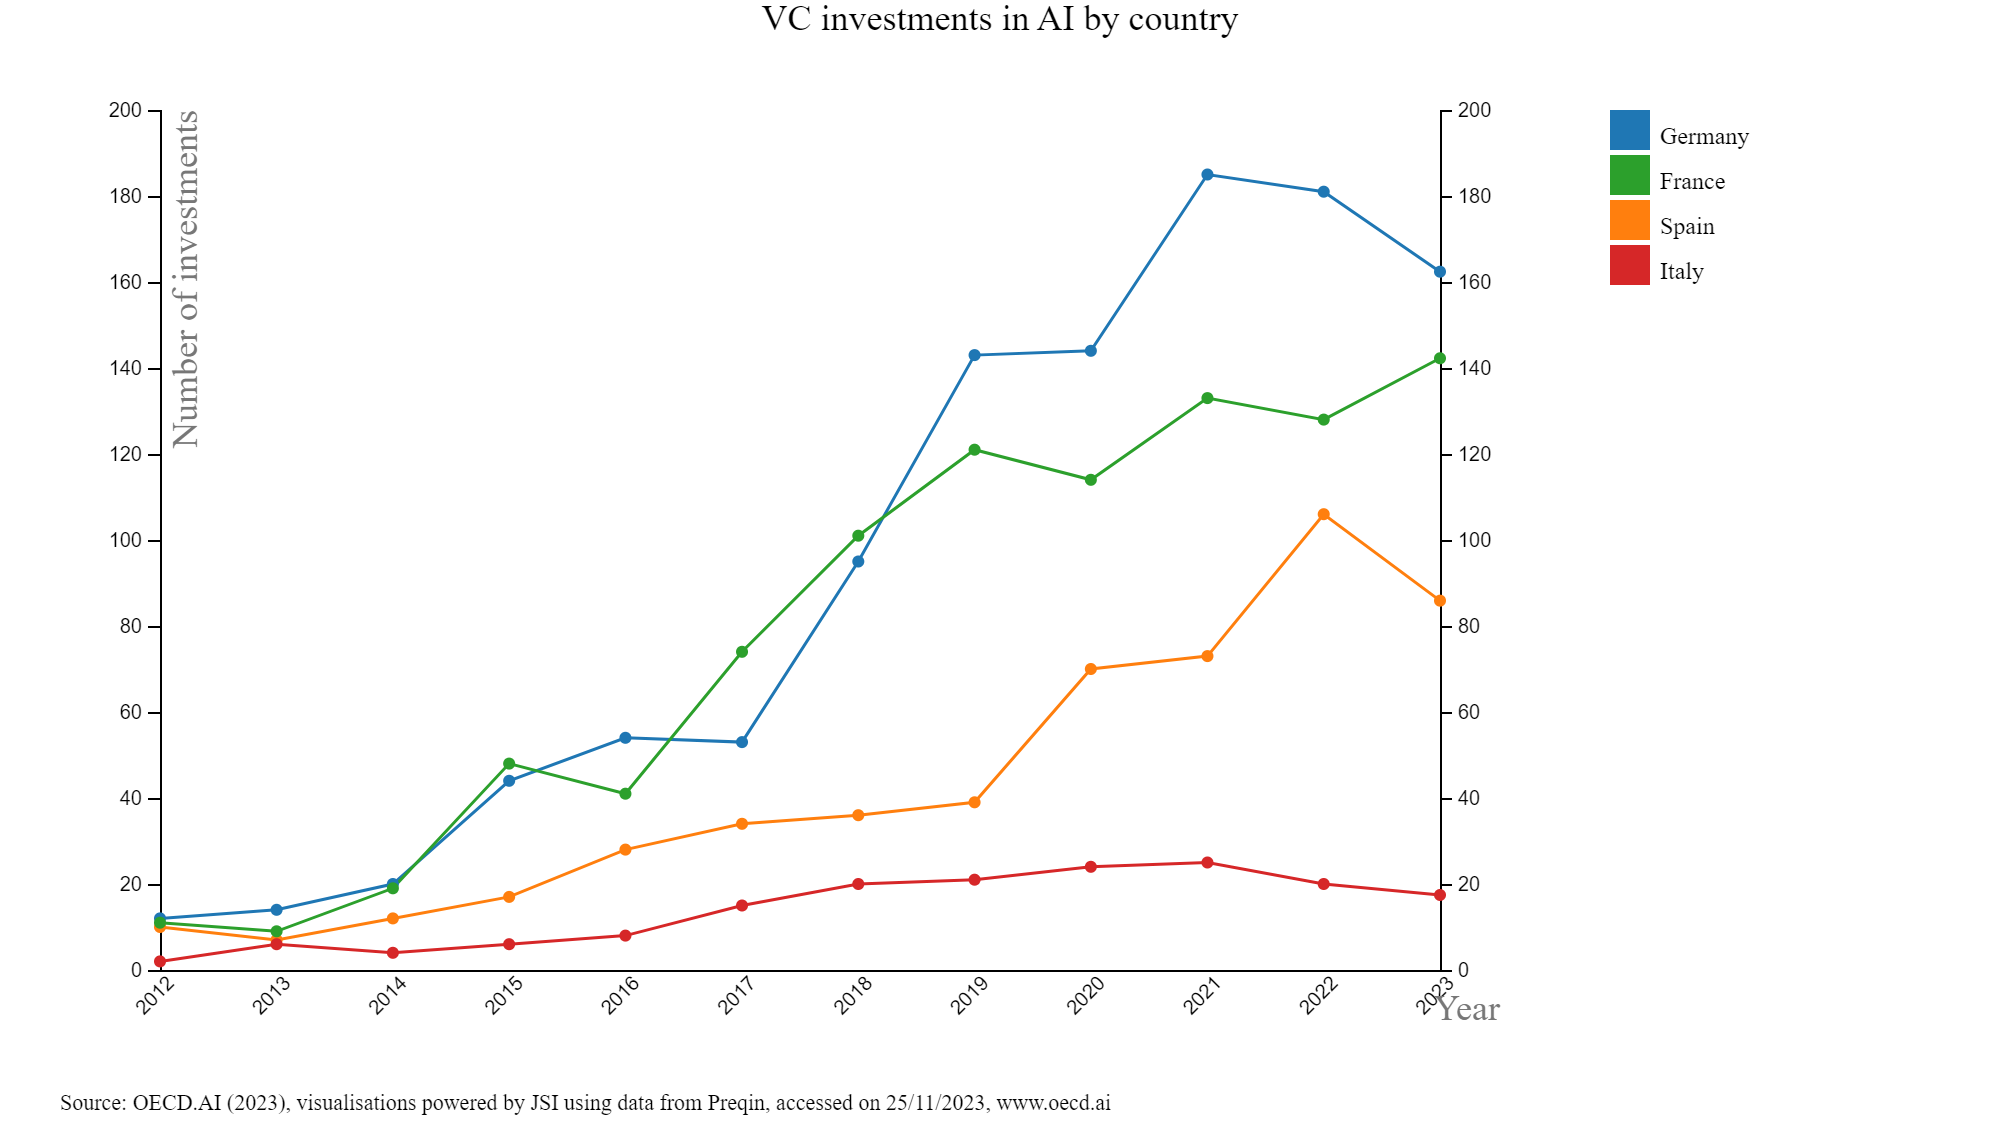
\includegraphics[width=0.3\linewidth]{Numero investimenti.png}
\end{center}
\begin{justify}
    Questo grafico rappresenta il numero degli investimenti effettuati per Stato nel settore AI e Data.
\end{justify}

\begin{center}
    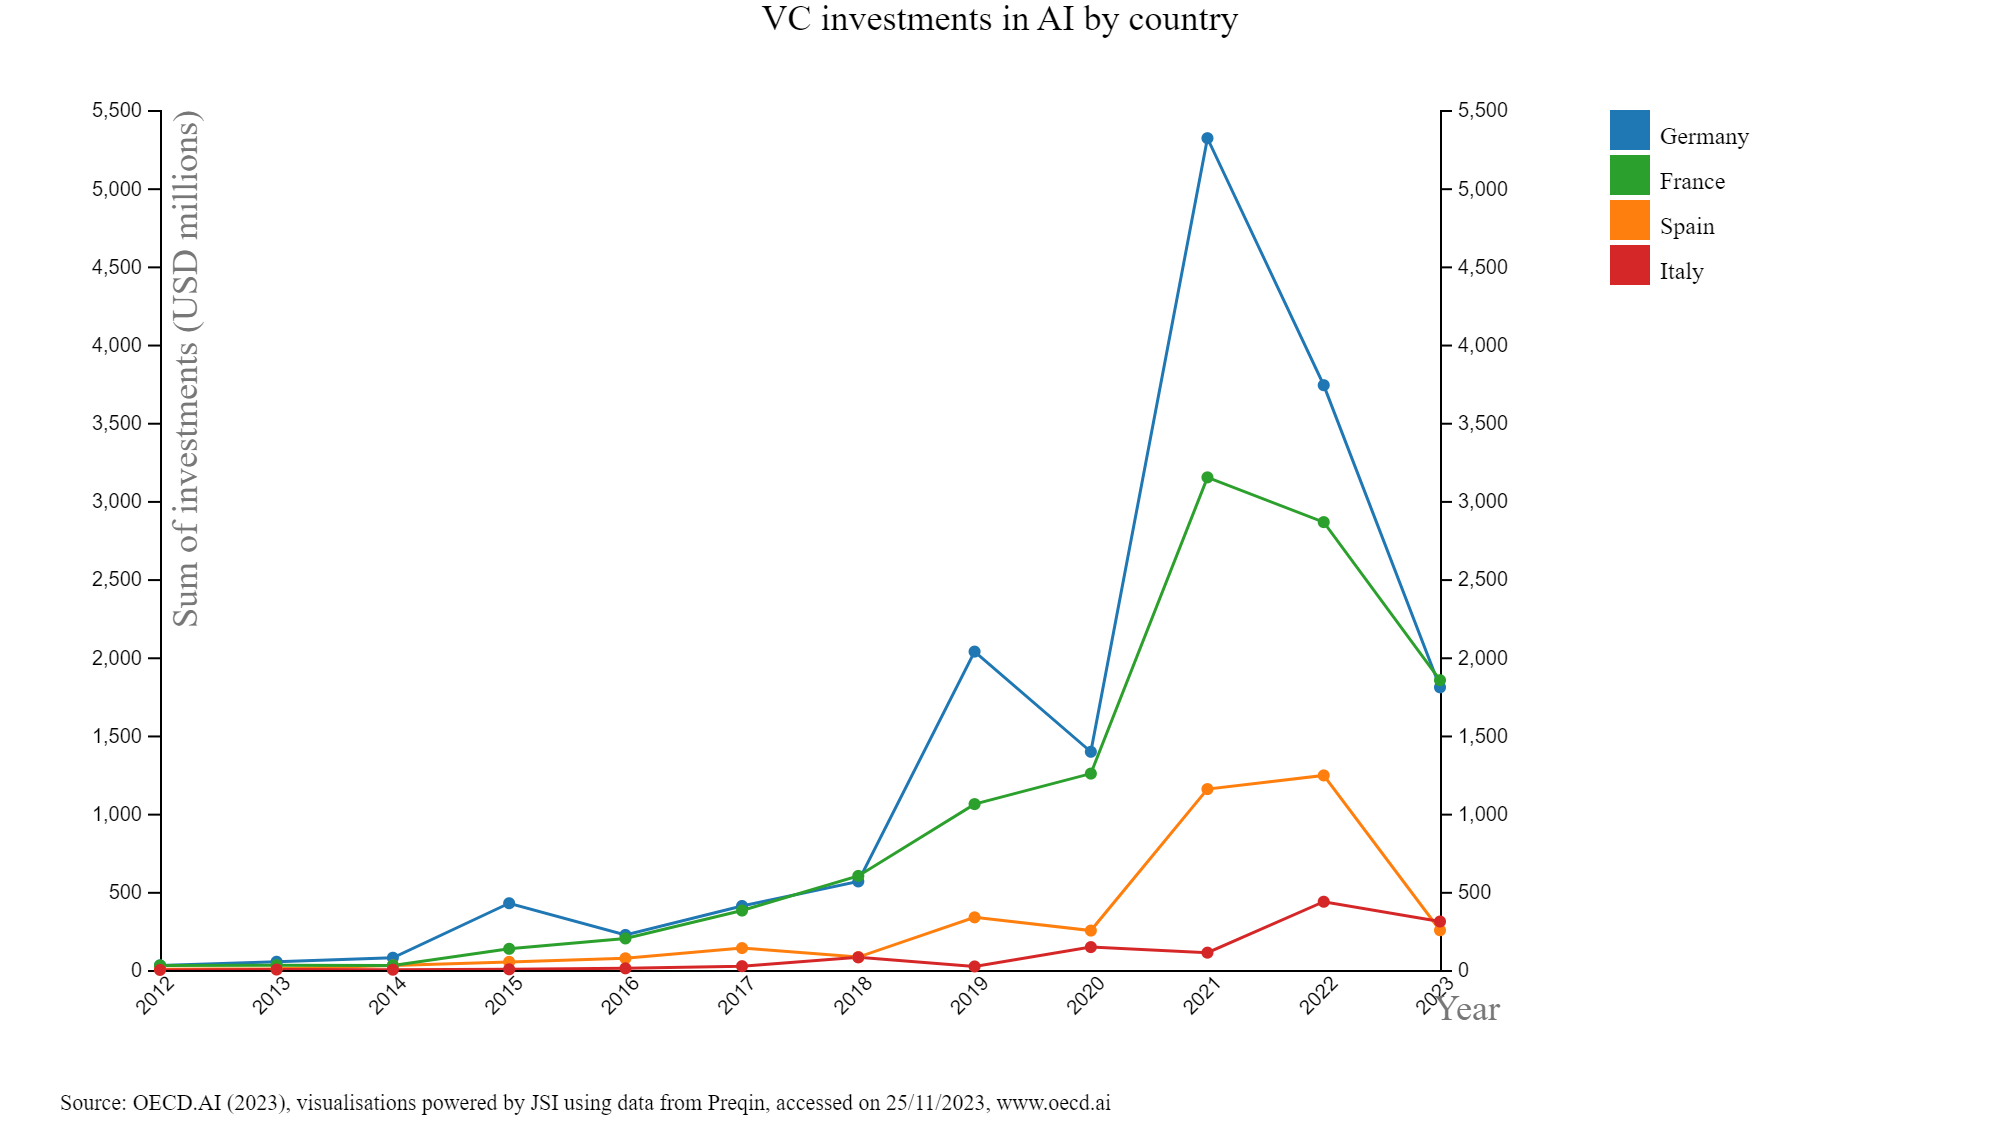
\includegraphics[width=0.3\linewidth]{Somma degli investimenti.png}
\end{center}
\begin{justify}
    Questo invece lo rappresenta sulla base dei milioni di dollari spesi in questo settore.
\end{justify}

\newpage \centering
\section{Conclusioni e opinioni finali}
\begin{justify}
   
\end{justify}

\begin{justify}
    \bibliography{Bibliografia}
    \bibliographystyle{plainnat}
\end{justify}
\end{document}